\section{Příklad 3}
% Jako parametr zadejte skupinu (A-H)
\tretiZadani{A}

\begin{center}
    \begin{LARGE}
        Řešení metodou uzlových napětí
    \end{LARGE}
\end{center}
\setcounter{figure}{0}

% Krok 1
\begin{itemize}
    \item Převedeme zdroj napětí na proudový zdroj a označíme uzly
\end{itemize}

\begin{figure}[h]
    \centering
    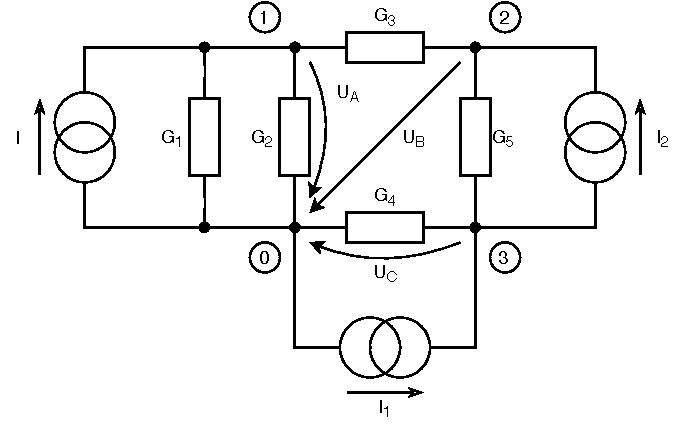
\includegraphics[scale=0.8,keepaspectratio]{fig/Pr3_krok1.pdf}
    \caption{Upravený obvod}
    \label{pic:Pr3_krok1}
\end{figure}

\begin{center}
    \begin{gather*}
        I = \frac{U}{R_1} = \frac{120}{53} \: A
    \end{gather*}
\end{center}

\newpage

% Krok 2
\begin{itemize}
    \item Spočítame vodivosti $G_1$, $G_2$, $G_3$, $G_4$ a $G_5$
\end{itemize}

\begin{center}
    \begin{gather*}
        G_1 = \frac{1}{R_1} = \frac{1}{53} \: S , \;
        G_2 = \frac{1}{R_2} = \frac{1}{49} \: S , \;
        G_3 = \frac{1}{R_3} = \frac{1}{65} \: S \\
        G_4 = \frac{1}{R_4} = \frac{1}{39} \: S , \;
        G_5 = \frac{1}{R_5} = \frac{1}{32} \: S \\
    \end{gather*}
\end{center}

% Krok 3
\begin{itemize}
    \item Sestavíme matice pro výpočet $U_A$, $U_B$, $U_C$
\end{itemize}

\begin{center}
    \begin{gather*}
        \begin{pmatrix}
            G_1 + G_2 + G_3 & -G_3 & 0 \\[6pt]
            -G_3 & G_3 + G_5 & -G_5 \\[6pt]
            0 & -G_5 & G_4 + G_5
        \end{pmatrix} \times
        \begin{pmatrix}
            U_A \\[6pt]
            U_B \\[6pt]
            U_C
        \end{pmatrix} =
        \begin{pmatrix}
            I \\[6pt]
            I_1 \\[6pt]
            I_2 - I_1
        \end{pmatrix} \\[8pt]
        \begin{pmatrix}
            \dfrac{1}{53} + \dfrac{1}{49} + \dfrac{1}{65} & -\dfrac{1}{65} & 0 \\[8pt]
            -\dfrac{1}{65} & \dfrac{1}{65} + \dfrac{1}{32} & -\dfrac{1}{32} \\[8pt]
            0 & -\dfrac{1}{32} & \dfrac{1}{39} + \dfrac{1}{32}
        \end{pmatrix} \times
        \begin{pmatrix}
            U_A \\[8pt]
            U_B \\[8pt]
            U_C
        \end{pmatrix} =
        \begin{pmatrix}
            \dfrac{120}{53} \\[8pt]
            \dfrac{9}{10} \\[8pt]
            -\dfrac{2}{10}
        \end{pmatrix} \\[8pt]
        \begin{pmatrix}
            \dfrac{3185+3445+2597}{168805} & -\dfrac{1}{65} & 0 \\[8pt]
            -\dfrac{1}{65} & \dfrac{32+65}{2080} & -\dfrac{1}{32} \\[8pt]
            0 & -\dfrac{1}{32} & \dfrac{32+39}{1248}
        \end{pmatrix} \times
        \begin{pmatrix}
            U_A \\[8pt]
            U_B \\[8pt]
            U_C
        \end{pmatrix} =
        \begin{pmatrix}
            \dfrac{120}{53} \\[8pt]
            \dfrac{9}{10} \\[8pt]
            -\dfrac{2}{10}
        \end{pmatrix} \\[8pt]
        \begin{pmatrix}
            \dfrac{9227}{168805} & -\dfrac{1}{65} & 0 \\[8pt]
            -\dfrac{1}{65} & \dfrac{97}{2080} & -\dfrac{1}{32} \\[8pt]
            0 & -\dfrac{1}{32} & \dfrac{71}{1248}
        \end{pmatrix} \times
        \begin{pmatrix}
            U_A \\[8pt]
            U_B \\[8pt]
            U_C
        \end{pmatrix} =
        \begin{pmatrix}
            \dfrac{120}{53} \\[8pt]
            \dfrac{9}{10} \\[8pt]
            -\dfrac{2}{10}
        \end{pmatrix}
    \end{gather*}
\end{center}

\newpage

% Krok 4
\begin{itemize}
    \item Spočítáme $U_A$ pomoci Cramerova pravidla
\end{itemize}

\begin{center}
    \begin{gather*}
        A = 
        \begin{pmatrix}
            \dfrac{9227}{168805} & -\dfrac{1}{65} & 0 \\[8pt]
            -\dfrac{1}{65} & \dfrac{97}{2080} & -\dfrac{1}{32} \\[8pt]
            0 & -\dfrac{1}{32} & \dfrac{71}{1248}
        \end{pmatrix} \;
        A_1 =
        \begin{pmatrix}
            \dfrac{120}{53} & -\dfrac{1}{65} & 0 \\[8pt]
            \dfrac{9}{10} & \dfrac{97}{2080} & -\dfrac{1}{32} \\[8pt]
            -\dfrac{2}{10} & -\dfrac{1}{32} & \dfrac{71}{1248}
        \end{pmatrix} \\[8pt]
        \lvert A\rvert = \frac{9227}{168805} \times \frac{97}{2080} \times \frac{71}{1248} - \frac{9227}{168805} \times \left( -\frac{1}{32}\right)^2 - \left( -\frac{1}{65}\right)^2 \times \frac{71}{1248} = \frac{16469}{210668640} \\[8pt]
        \lvert A_1\rvert = \frac{120}{53} \times \frac{97}{2080} \times \frac{71}{1248} + \left( -\frac{2}{10}\right) \times \left( -\frac{1}{65}\right) \times \left( -\frac{1}{32}\right) - \\[8pt]
        - \frac{120}{53} \times \left( -\frac{1}{32}\right)^2 - \frac{9}{10} \times \left( -\frac{1}{65}\right) \times \frac{71}{1248} = \frac{4947}{1102400} \\[8pt]
        U_A = \frac{\lvert A\rvert}{\lvert A_1\rvert} = \frac{\dfrac{4947}{1102400}}{\dfrac{16469}{210668640}} = \frac{4947}{1102400} \times \frac{210668640}{16469} = 57,4031 \: V \\
    \end{gather*}
\end{center}

% Krok 5
\begin{itemize}
    \item $U_A$ se rovná $U_{R_2}$ (podle obrázku), tedy můžeme spočítat $I_{R_2}$ (Ohmův zákon)
\end{itemize}

\begin{center}
    \begin{gather*}
        U_A = U_{R_2} = 57,4031 \: V \\[8pt]
        I_{R_2} = \frac{U_{R_2}}{R_2} = \frac{57,4031}{49} = 1,1715 \: V
    \end{gather*}
\end{center}